% move all configuration stuff into includes file so we can focus on the content
\documentclass[aspectratio=169,hyperref={pdfpagelabels=false,colorlinks=true,linkcolor=white,urlcolor=blue},t]{beamer}

%%%%%%%%%%%%%%%%%%%%%%%%%%%%%%%%%%%%%%%%%%%%%%%%%%%%%%%%%%%%%%%%%%%%%%%%%%%%%%%%%%
%%%%%%%%%%%%%%%%%%%%%%%%%%%%%%%%%%%%%%%%%%%%%%%%%%%%%%%%%%%%%%%%%%%%%%%%%%%%%%%%%%
% packages
\usepackage{pict2e}
\usepackage{epic}
\usepackage{amsmath,amsfonts,amssymb}
\usepackage{units}
\usepackage{fancybox}
\usepackage[absolute,overlay]{textpos} 
\usepackage{media9} % avi2flv: "C:\Program Files\ffmpeg\bin\ffmpeg.exe" -i TuneFreqFilterbank.avi -b 600k -s 441x324 -r 15 -acodec copy TuneFreqFilterbank.flv
\usepackage{animate}
\usepackage{gensymb}
\usepackage{multirow}
\usepackage{silence}
\usepackage{tikz}
\usepackage[backend=bibtex,style=ieee]{biblatex}
\AtEveryCitekey{\iffootnote{\tiny}{}}
\addbibresource{include/references}

%%%%%%%%%%%%%%%%%%%%%%%%%%%%%%%%%%%%%%%%%%%%%%%%%%%%%%%%%%%%%%%%%%%%%%%%%%%%%%%%%%
%%%%%%%%%%%%%%%%%%%%%%%%%%%%%%%%%%%%%%%%%%%%%%%%%%%%%%%%%%%%%%%%%%%%%%%%%%%%%%%%%%
% relative paths
\graphicspath{{graph/}}


%%%%%%%%%%%%%%%%%%%%%%%%%%%%%%%%%%%%%%%%%%%%%%%%%%%%%%%%%%%%%%%%%%%%%%%%%%%%%%%%%%
%%%%%%%%%%%%%%%%%%%%%%%%%%%%%%%%%%%%%%%%%%%%%%%%%%%%%%%%%%%%%%%%%%%%%%%%%%%%%%%%%%
% units
\setlength{\unitlength}{1mm}

%%%%%%%%%%%%%%%%%%%%%%%%%%%%%%%%%%%%%%%%%%%%%%%%%%%%%%%%%%%%%%%%%%%%%%%%%%%%%%%%%%
%%%%%%%%%%%%%%%%%%%%%%%%%%%%%%%%%%%%%%%%%%%%%%%%%%%%%%%%%%%%%%%%%%%%%%%%%%%%%%%%%%
% theme & layout
\usetheme{Frankfurt}
\beamertemplatenavigationsymbolsempty
%\setbeamertemplate{frametitle}[smoothbars theme]
\setbeamertemplate{frametitle}
{
    \begin{beamercolorbox}[ht=1.8em,wd=\paperwidth]{frametitle}
        \vspace{-.1em}%
        \hspace{.2em}{\strut\insertframetitle\strut}
        
        \hspace{.2em}\small\strut\insertframesubtitle\strut
        %\hfill
        %\includegraphics[height=.8cm,keepaspectratio]{CenterMusicTechnology-solid-2lines-white-CoAtag}
        
    \end{beamercolorbox}
    \begin{textblock*}{100mm}(11.6cm,.7cm)
        \includegraphics[height=.8cm,keepaspectratio]{Logo_GTCMT_black}
    \end{textblock*}
}
\setbeamertemplate{footline}[frame number]

% set this to ensure bulletpoints without subsections
\usepackage{remreset}
\makeatletter
\@removefromreset{subsection}{section}
\makeatother
\setcounter{subsection}{1}

%---------------------------------------------------------------------------------
% appearance
\setbeamercolor{structure}{fg=gtgold}
\setbeamercovered{transparent} %invisible
\setbeamercolor{bibliography entry author}{fg=black}
\setbeamercolor*{bibliography entry title}{fg=black}
\setbeamercolor*{bibliography entry note}{fg=black}
\setbeamercolor{frametitle}{fg=black}
\setbeamercolor{title}{fg=black}

%\usepackage{pgfpages}
%\setbeameroption{show notes}
%\setbeameroption{show notes on second screen=right}
%---------------------------------------------------------------------------------
% fontsize
\let\Tiny=\tiny

%%%%%%%%%%%%%%%%%%%%%%%%%%%%%%%%%%%%%%%%%%%%%%%%%%%%%%%%%%%%%%%%%%%%%%%%%%%%%%%%%%
%%%%%%%%%%%%%%%%%%%%%%%%%%%%%%%%%%%%%%%%%%%%%%%%%%%%%%%%%%%%%%%%%%%%%%%%%%%%%%%%%%
% warnings
\pdfsuppresswarningpagegroup=1
\WarningFilter{biblatex}{Patching footnotes failed}
\WarningFilter{latexfont}{Font shape}
\WarningFilter{latexfont}{Some font shapes}
\WarningFilter{gensymb}{Not defining}


%%%%%%%%%%%%%%%%%%%%%%%%%%%%%%%%%%%%%%%%%%%%%%%%%%%%%%%%%%%%%%%%%%%%%%%%%%%%%%%%%%
%%%%%%%%%%%%%%%%%%%%%%%%%%%%%%%%%%%%%%%%%%%%%%%%%%%%%%%%%%%%%%%%%%%%%%%%%%%%%%%%%%
% theme & layout
\usetheme{Frankfurt}
\useinnertheme{rectangles}


%%%%%%%%%%%%%%%%%%%%%%%%%%%%%%%%%%%%%%%%%%%%%%%%%%%%%%%%%%%%%%%%%%%%%%%%%%%%%%%%%%
\setbeamertemplate{frametitle}[default][colsep=-4bp,rounded=false,shadow=false]
\setbeamertemplate{frametitle}
{%
    \nointerlineskip%
    %\vskip-0.5ex
    \begin{beamercolorbox}[wd=\paperwidth,ht=3.5ex,dp=0.6ex]{frametitle}
        \hspace*{1.3ex}\insertframetitle%
        
        \hspace*{1.3ex}\small\insertframesubtitle%
    \end{beamercolorbox}%
    \begin{textblock*}{100mm}(11.6cm,.57cm)
        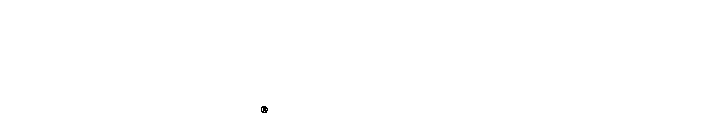
\includegraphics[height=.8cm,keepaspectratio]{graph/Logo_GTCMT_white}
    \end{textblock*}
}


%%%%%%%%%%%%%%%%%%%%%%%%%%%%%%%%%%%%%%%%%%%%%%%%%%%%%%%%%%%%%%%%%%%%%%%%%%%%%%%%%%
\setbeamertemplate{title page}[default][colsep=-4bp,rounded=false,shadow=false]
\setbeamertemplate{title page}
{
    \begin{textblock*}{100mm}(15cm,.51cm)
            \href{https://github.com/alexanderlerch/ACA-Slides/blob/2nd_edition/\jobname.pdf}{\includegraphics[height=.5cm,keepaspectratio]{graph/Logo_github}}\hspace*{2ex}
    \end{textblock*}
    \vskip-10ex
    \begin{beamercolorbox}[wd=\paperwidth,ht=.7\paperheight,dp=0.6ex]{frametitle} %35ex
        %\begin{flushright}
            %\href{http://www.gtcmt.gatech.edu}{\includegraphics[height=.8cm,keepaspectratio]{graph/Logo_GTCMT_black}}\hspace*{2ex}
        %\end{flushright}
        
        \hspace*{1.8ex}\LARGE\inserttitle%
        
        \vspace*{.5ex}
        
        \hspace*{1.3ex}\small\insertsubtitle%
        
        \vspace*{.5ex}
    \end{beamercolorbox}%
    \nointerlineskip%
    \begin{beamercolorbox}[wd=\paperwidth,ht=.4\paperheight,dp=0.6ex]{page number in head/foot}
        %\vspace*{-.5ex}
        \hspace*{1.7ex}\small\insertauthor%
        
        %\hspace*{1.7ex}\small }%
        
        \vspace*{10ex}
        
        \begin{flushright}
            \href{http://www.gtcmt.gatech.edu}{\includegraphics[height=.8cm,keepaspectratio]{graph/Logo_GTCMT_black}}\hspace*{2ex}
        \end{flushright}
    \end{beamercolorbox}%
}


%%%%%%%%%%%%%%%%%%%%%%%%%%%%%%%%%%%%%%%%%%%%%%%%%%%%%%%%%%%%%%%%%%%%%%%%%%%%%%%%%%
%\makeatother
\setbeamertemplate{footline}
{
  \leavevmode%
  \hbox{%
  \begin{beamercolorbox}[wd=.5\paperwidth,ht=2.25ex,dp=1ex,left,leftskip=1ex]{page number in head/foot}%
    \insertsubtitle
  \end{beamercolorbox}%
  \begin{beamercolorbox}[wd=.5\paperwidth,ht=2.25ex,dp=1ex,right,rightskip=1ex]{page number in head/foot}%
    \hfill
    \insertframenumber{} / \inserttotalframenumber
  \end{beamercolorbox}}%
  \vskip0pt%
}
%\makeatletter


%%%%%%%%%%%%%%%%%%%%%%%%%%%%%%%%%%%%%%%%%%%%%%%%%%%%%%%%%%%%%%%%%%%%%%%%%%%%%%%%%%
\beamertemplatenavigationsymbolsempty
\setbeamertemplate{navigation symbols}{}
\setbeamertemplate{blocks}[default]%[rounded=false,shadow=false]
\setbeamertemplate{itemize item}[square]
\setbeamertemplate{itemize subitem}[circle]
\setbeamertemplate{itemize subsubitem}[triangle]
\setbeamertemplate{enumerate item}[square]
\setbeamertemplate{enumerate subitem}[circle]
\setbeamertemplate{enumerate subsubitem}[circle]


%%%%%%%%%%%%%%%%%%%%%%%%%%%%%%%%%%%%%%%%%%%%%%%%%%%%%%%%%%%%%%%%%%%%%%%%%%%%%%%%%%
% colors
\setbeamercolor{structure}{fg=darkgray}
\setbeamercovered{transparent} %invisible
\setbeamercolor{bibliography entry author}{fg=black}
\setbeamercolor*{bibliography entry title}{fg=black}
\setbeamercolor*{bibliography entry note}{fg=black}
\setbeamercolor{frametitle}{fg=black}
\setbeamercolor{title}{fg=white}
\setbeamercolor{subtitle}{fg=white}
\setbeamercolor{frametitle}{fg=white}
\setbeamercolor{framesubtitle}{fg=white}
\setbeamercolor{mini frame}{fg=white, bg=black}
\setbeamercolor{section in head/foot}{fg=white, bg=darkgray}
\setbeamercolor{page number in head/foot}{fg=black, bg=lightblue}
\setbeamercolor{item projected}{fg=white, bg=black}

%---------------------------------------------------------------------------------
%%%%%%%%%%%%%%%%%%%%%%%%%%%%%%%%%%%%%%%%%%%%%%%%%%%%%%%%%%%%%%%%%%%%%%%%%%%%%%%%%%
%%%%%%%%%%%%%%%%%%%%%%%%%%%%%%%%%%%%%%%%%%%%%%%%%%%%%%%%%%%%%%%%%%%%%%%%%%%%%%%%%%
% title information
\title[]{Introduction to \textbf{Audio Content Analysis}}   
\author[alexander lerch]{alexander lerch} 
%\institute{~}
%\date[Alexander Lerch]{}
%\titlegraphic{\vspace{-16mm}\includegraphics[width=\textwidth,height=3cm]{title}}

%%%%%%%%%%%%%%%%%%%%%%%%%%%%%%%%%%%%%%%%%%%%%%%%%%%%%%%%%%%%%%%%%%%%%%%%%%%%%%%%%%
%%%%%%%%%%%%%%%%%%%%%%%%%%%%%%%%%%%%%%%%%%%%%%%%%%%%%%%%%%%%%%%%%%%%%%%%%%%%%%%%%%
% colors
\definecolor{gtgold}{HTML}{E0AA0F} %{rgb}{0.88,0.66,1,0.06} [234, 170, 0]/256
\definecolor{darkgray}{rgb}{.1, .1, .25}
\definecolor{lightblue}{rgb}{.1, 0.75, 1}
\definecolor{highlight}{rgb}{0, 0, 1} %_less!40

%%%%%%%%%%%%%%%%%%%%%%%%%%%%%%%%%%%%%%%%%%%%%%%%%%%%%%%%%%%%%%%%%%%%%%%%%%%%%%%%%%
%%%%%%%%%%%%%%%%%%%%%%%%%%%%%%%%%%%%%%%%%%%%%%%%%%%%%%%%%%%%%%%%%%%%%%%%%%%%%%%%%%
% relative paths
\graphicspath{{../ACA-Plots/graph/}}


%%%%%%%%%%%%%%%%%%%%%%%%%%%%%%%%%%%%%%%%%%%%%%%%%%%%%%%%%%%%%%%%%%%%%%%%%%%%%%%%%%
%%%%%%%%%%%%%%%%%%%%%%%%%%%%%%%%%%%%%%%%%%%%%%%%%%%%%%%%%%%%%%%%%%%%%%%%%%%%%%%%%%
% units
\setlength{\unitlength}{1mm}

%%%%%%%%%%%%%%%%%%%%%%%%%%%%%%%%%%%%%%%%%%%%%%%%%%%%%%%%%%%%%%%%%%%%%%%%%%%%%%%%%%
%%%%%%%%%%%%%%%%%%%%%%%%%%%%%%%%%%%%%%%%%%%%%%%%%%%%%%%%%%%%%%%%%%%%%%%%%%%%%%%%%%
% math
\DeclareMathOperator*{\argmax}{argmax}
\DeclareMathOperator*{\argmin}{argmin}
\DeclareMathOperator*{\atan}{atan}
\DeclareMathOperator*{\arcsinh}{arcsinh}
\DeclareMathOperator*{\sign}{sign}
\DeclareMathOperator*{\tcdf}{tcdf}
\DeclareMathOperator*{\si}{sinc}
\DeclareMathOperator*{\princarg}{princarg}
\DeclareMathOperator*{\arccosh}{arccosh}
\DeclareMathOperator*{\hwr}{HWR}
\DeclareMathOperator*{\flip}{flip}
\DeclareMathOperator*{\sinc}{sinc}
\DeclareMathOperator*{\floor}{floor}
\newcommand{\e}{{e}}
\newcommand{\jom}{\mathrm{j}\omega}
\newcommand{\jOm}{\mathrm{j}\Omega}
\newcommand   {\mat}[1]    		{\boldsymbol{\uppercase{#1}}}		%bold
\renewcommand {\vec}[1]    		{\boldsymbol{\lowercase{#1}}}		%bold

%%%%%%%%%%%%%%%%%%%%%%%%%%%%%%%%%%%%%%%%%%%%%%%%%%%%%%%%%%%%%%%%%%%%%%%%%%%%%%%%%%
%%%%%%%%%%%%%%%%%%%%%%%%%%%%%%%%%%%%%%%%%%%%%%%%%%%%%%%%%%%%%%%%%%%%%%%%%%%%%%%%%%
% media9
\newcommand{\includeaudio}[1]{
\href{run:audio/#1.mp3}{
\includegraphics[width=5mm, height=5mm]{graph/SpeakerIcon}}}

\newcommand{\includeanimation}[4]{{\begin{center}
                        \animategraphics[autoplay,loop,scale=.7]{#4}{animation/#1-}{#2}{#3}        
                        \end{center}
                        \addreference{matlab source: \href{https://github.com/alexanderlerch/ACA-Plots/blob/master/matlab/animate#1.m}{matlab/animate#1.m}}}
                        \inserticon{video}}
                        
%%%%%%%%%%%%%%%%%%%%%%%%%%%%%%%%%%%%%%%%%%%%%%%%%%%%%%%%%%%%%%%%%%%%%%%%%%%%%%%%%%
%%%%%%%%%%%%%%%%%%%%%%%%%%%%%%%%%%%%%%%%%%%%%%%%%%%%%%%%%%%%%%%%%%%%%%%%%%%%%%%%%%
% other commands
\newcommand{\question}[1]{%\vspace{-4mm}
                          \setbeamercovered{invisible}
                          \begin{columns}[T]
                            \column{.9\textwidth}
                                \textbf{#1}
                            \column{.1\textwidth}
                                \vspace{-8mm}
                                \begin{flushright}
                                     
\includegraphics[width=.9\columnwidth]{graph/question_mark}
                                \end{flushright}
                                \vspace{6mm}
                          \end{columns}\pause\vspace{-12mm}}

\newcommand{\toremember}[1]{
                        \inserticon{lightbulb}
                        }

\newcommand{\matlabexercise}[1]{%\vspace{-4mm}
                          \setbeamercovered{invisible}
                          \begin{columns}[T]
                            \column{.8\textwidth}
                                \textbf{matlab exercise}: #1
                            \column{.2\textwidth}
                                \begin{flushright}
                                     \includegraphics[scale=.5]{graph/logo_matlab}
                                \end{flushright}
                                %\vspace{6mm}
                          \end{columns}}

\newcommand{\addreference}[1]{  
                  
                    \begin{textblock*}{\baselineskip }(.98\paperwidth,.5\textheight) %(1.15\textwidth,.4\textheight)
                         \begin{minipage}[b][.5\paperheight][b]{1cm}%
                            \vfill%
                             \rotatebox{90}{\tiny {#1}}
                        \end{minipage}
                   \end{textblock*}
                    }
                    
\newcommand{\figwithmatlab}[1]{
                    \begin{figure}
                        \centering
                        \includegraphics[scale=.7]{#1}
                        %\label{fig:#1}
                    \end{figure}
                    
                    \addreference{matlab source: \href{https://github.com/alexanderlerch/ACA-Plots/blob/main/matlab/plot#1.m}{plot#1.m}}}
\newcommand{\figwithref}[2]{
                    \begin{figure}
                        \centering
                        \includegraphics[scale=.7]{#1}
                        \label{fig:#1}
                    \end{figure}
                    
                    \addreference{#2}}  
                                    
\newcommand{\inserticon}[1]{
                    \begin{textblock*}{100mm}(14.5cm,7.5cm)
                        \includegraphics[height=.8cm,keepaspectratio]{graph/#1}
                    \end{textblock*}}            

%%%%%%%%%%%%%%%%%%%%%%%%%%%%%%%%%%%%%%%%%%%%%%%%%%%%%%%%%%%%%%%%%%%%%%%%%%%%%%%%%%
%%%%%%%%%%%%%%%%%%%%%%%%%%%%%%%%%%%%%%%%%%%%%%%%%%%%%%%%%%%%%%%%%%%%%%%%%%%%%%%%%%
% counters
\newcounter{i}
\newcounter{j}
\newcounter{iXOffset}
\newcounter{iYOffset}
\newcounter{iXBlockSize}
\newcounter{iYBlockSize}
\newcounter{iYBlockSizeDiv2}
\newcounter{iXBlockSizeDiv2}
\newcounter{iDistance}




\subtitle{module 5.0: data, data splits, and augmentation}

%%%%%%%%%%%%%%%%%%%%%%%%%%%%%%%%%%%%%%%%%%%%%%%%%%%%%%%%%%%%%%%%%%%%%%%%%%%%
\begin{document}
    % generate title page
	{
\setbeamertemplate{headline}{} 
\setbeamertemplate{footline}{} 
\begin{frame}
    \titlepage
    %\vspace{-5mm}
\end{frame}
}
\addtocounter{framenumber}{-1}


    \section[overview]{lecture overview}
        \begin{frame}{introduction}{overview}
            \begin{block}{corresponding textbook section}
                    %\href{http://ieeexplore.ieee.org/xpl/articleDetails.jsp?arnumber=6331125}{Chapter 8: Musical Genre, Similarity, and Mood} (pp.~155)
                    chapter~5
            \end{block}

            \begin{itemize}
                \item   \textbf{lecture content}
                    \begin{itemize}
                        \item   data requirements
                        \item   data splits for train and test
                        \item   N-Fold cross-validation
                        \item   data augmentation
                    \end{itemize}
                \bigskip
                \item<2->   \textbf{learning objectives}
                    \begin{itemize}
                        \item   understand the importance of data in machine learning 
                        \item   define task-specific data requirements
                        \item   discuss possibilities of data augmentation
                        \item   implement N-Fold cross-validation in Python
                    \end{itemize}
            \end{itemize}
            \inserticon{directions}
        \end{frame}

    \section[intro]{introduction}
        \begin{frame}{machine learning}{data-driven}
           \begin{itemize}
                \item   derive classification parameters from data, e.g.,
                \item[$\Rightarrow$]  learn feature distributions/separation metrics per class
                \bigskip
                \item  typical steps
                    \begin{enumerate}
                        \item	\textbf{define training set}: annotated results
                        \smallskip
                        \item<2->	\textbf{normalize} training set
                        \smallskip
                        \item<3->	\textbf{train} classifier
                        \smallskip
                        \item<4->	\textbf{evaluate} classifier with test (or validation) set
                        \smallskip
                        \item<5->	(\textbf{adjust} classifier settings, return to 4.)
                    \end{enumerate}
            \end{itemize}
        \end{frame}

    \section{data}
        \begin{frame}{data}{requirements}
            \question{what are important properties of our data} 
          
            \begin{itemize}
                \item   \textbf{representative}
                    \begin{itemize}
                        \item   represent all necessary factors of input data (e.g., range of genres, audio qualities, musical complexity, etc.)
                        \item   unbiased representation of class balance/label distribution
                    \end{itemize}
                \smallskip
                \item   \textbf{clean}, non-noisy
                    \begin{itemize}
                        \item   potential issues with subjective tasks
                    \end{itemize}
                \smallskip
                \item   \textbf{sufficient}
                    \begin{itemize}
                        \item   complex tasks/systems require lots of data
                    \end{itemize}
            \end{itemize}
        \end{frame}
        
        \begin{frame}{data}{data split}
            \vspace{-5mm}
            \begin{columns}
            \column{.6\linewidth}
            \begin{itemize}
                \item   a bigger data set is commonly split in subsets
                    \smallskip
                    \begin{itemize}
                        \item   \textbf{training data} ($\approx 70-80\%$)
                            \begin{itemize}
                                \item   used to build the machine learning model
                            \end{itemize}
                        \smallskip
                        \item   \textbf{validation data }($\approx 10-15\%$)
                            \begin{itemize}
                                \item   used to tweak model parameters
                            \end{itemize}
                        \smallskip
                        \item   \textbf{testing data} ($\approx 10-15\%$)
                            \begin{itemize}
                                \item   used to evaluate the model
                                \item   needs to be \textbf{unseen}!
                            \end{itemize}
                    \end{itemize}
                \bigskip
                \pause
                \item   no overlap between subsets!
                    \begin{itemize}
                        \item also make sure that similar content (from one recording, album, artist, ...) is grouped into \textbf{one subset only}
                    \end{itemize}
            \end{itemize}
            \column{.6\linewidth}
                \figwithmatlab{DataSplit}
            \end{columns}
        \end{frame}
        
        \begin{frame}{data}{N-Fold cross validation 1/2}

            \begin{itemize}
                \item   trying to utilize ALL data as both training and testing data
                \item   special case: Leave One Out CV
                \item   tends to be time-consuming
            \end{itemize}
            \bigskip
            \begin{enumerate}
                \item<2->	split training set into $N$ parts (randomly, but preferably identical number per class)
                \item<3->	select one part as test set
                \item<4->	train the classifier with all observations from remaining $N-1$ parts
                \item<5->	compute the classification rate for the test set
                \item<6->	repeat until all $N$ parts have been tested
                \item<7->	overall result: \textit{average} classification rate
            \end{enumerate}
        \end{frame}
        
        \begin{frame}{data}{N-Fold cross validation 2/2}
            \begin{figure}
                \begin{footnotesize}
    \begin{picture}(90,36)
        {\setlength\fboxsep{0pt}
        \setcounter{iXOffset}{2}
        \setcounter{iYOffset}{25}
        \setcounter{iXBlockSize}{80}
        \setcounter{iYBlockSize}{4}
        \setcounter{iYBlockSizeDiv2}{2}
        \setcounter{iXBlockSizeDiv2}{20}
        \setcounter{iDistance}{8}

        % block indices
        \addtocounter{iYOffset}{-\value{iYBlockSize}}
        \addtocounter{iYOffset}{-\value{iYBlockSizeDiv2}}
        \put(\value{iXOffset}, \value{iYOffset})
            {\text{{\shortstack[c]{1.}}}}
        \addtocounter{iYOffset}{-\value{iYBlockSize}}
        \addtocounter{iYOffset}{-\value{iYBlockSizeDiv2}}
        \put(\value{iXOffset}, \value{iYOffset})
            {\text{{\shortstack[c]{2.}}}}
        \addtocounter{iYOffset}{-\value{iYBlockSize}}
        \addtocounter{iYOffset}{-\value{iYBlockSizeDiv2}}
        \put(\value{iXOffset}, \value{iYOffset})
            {\text{{\shortstack[c]{3.}}}}
        \addtocounter{iYOffset}{-\value{iYBlockSize}}
        \addtocounter{iYOffset}{-\value{iYBlockSizeDiv2}}
        \put(\value{iXOffset}, \value{iYOffset})
            {\text{{\shortstack[c]{4.}}}}

        \setcounter{iYOffset}{30}
        \addtocounter{iXOffset}{\value{iDistance}}
        % data
        \put(\value{iXOffset}, \value{iYOffset})
            {\framebox(\value{iXBlockSize}, \value{iYBlockSize}){Data}}

        % blocks
        \addtocounter{iYOffset}{-\value{iYBlockSize}}
        \addtocounter{iYOffset}{-\value{iYBlockSizeDiv2}}
        \put(\value{iXOffset}, \value{iYOffset})
            {\framebox(\value{iXBlockSizeDiv2}, \value{iYBlockSize}){Split 1}}
        \addtocounter{iXOffset}{\value{iXBlockSizeDiv2}}
        \put(\value{iXOffset}, \value{iYOffset})
            {\framebox(\value{iXBlockSizeDiv2}, \value{iYBlockSize}){Split 2}}
        \addtocounter{iXOffset}{\value{iXBlockSizeDiv2}}
        \put(\value{iXOffset}, \value{iYOffset})
            {\framebox(\value{iXBlockSizeDiv2}, \value{iYBlockSize}){Split 3}}
        \addtocounter{iXOffset}{\value{iXBlockSizeDiv2}}
        \put(\value{iXOffset}, \value{iYOffset})
            {\framebox(\value{iXBlockSizeDiv2}, \value{iYBlockSize}){Split 4}}
        \addtocounter{iXOffset}{\value{iXBlockSizeDiv2}}
        \addtocounter{iXOffset}{-\value{iXBlockSize}}


        \addtocounter{iYOffset}{-\value{iYBlockSize}}
        \addtocounter{iYOffset}{-\value{iYBlockSizeDiv2}}
        \put(\value{iXOffset}, \value{iYOffset})
            {{\framebox(\value{iXBlockSizeDiv2}, \value{iYBlockSize}){Test}}}
            %{\framebox(\value{iXBlockSizeDiv2}, \value{iYBlockSize}){Test}}
        \addtocounter{iXOffset}{\value{iXBlockSizeDiv2}}
        \put(\value{iXOffset}, \value{iYOffset})
            {\colorbox{gray!10}{\framebox(\value{iXBlockSizeDiv2}, \value{iYBlockSize}){Train}}}
            %{\framebox(\value{iXBlockSizeDiv2}, \value{iYBlockSize}){Train}}
        \addtocounter{iXOffset}{\value{iXBlockSizeDiv2}}
        \put(\value{iXOffset}, \value{iYOffset})
            {\colorbox{gray!10}{\framebox(\value{iXBlockSizeDiv2}, \value{iYBlockSize}){Train}}}
            %{\framebox(\value{iXBlockSizeDiv2}, \value{iYBlockSize}){Train}}
        \addtocounter{iXOffset}{\value{iXBlockSizeDiv2}}
        \put(\value{iXOffset}, \value{iYOffset})
            {\colorbox{gray!10}{\framebox(\value{iXBlockSizeDiv2}, \value{iYBlockSize}){Train}}}
            %{\framebox(\value{iXBlockSizeDiv2}, \value{iYBlockSize}){Train}}
        \addtocounter{iXOffset}{\value{iXBlockSizeDiv2}}
        \addtocounter{iXOffset}{-\value{iXBlockSize}}


        \addtocounter{iYOffset}{-\value{iYBlockSize}}
        \addtocounter{iYOffset}{-\value{iYBlockSizeDiv2}}
        \put(\value{iXOffset}, \value{iYOffset})
            {\colorbox{gray!10}{\framebox(\value{iXBlockSizeDiv2}, \value{iYBlockSize}){Train}}}
            %{\framebox(\value{iXBlockSizeDiv2}, \value{iYBlockSize}){Train}}
        \addtocounter{iXOffset}{\value{iXBlockSizeDiv2}}
        \put(\value{iXOffset}, \value{iYOffset})
            {{\framebox(\value{iXBlockSizeDiv2}, \value{iYBlockSize}){Test}}}
            %{\framebox(\value{iXBlockSizeDiv2}, \value{iYBlockSize}){Test}}
        \addtocounter{iXOffset}{\value{iXBlockSizeDiv2}}
        \put(\value{iXOffset}, \value{iYOffset})
            {\colorbox{gray!10}{\framebox(\value{iXBlockSizeDiv2}, \value{iYBlockSize}){Train}}}
            %{\framebox(\value{iXBlockSizeDiv2}, \value{iYBlockSize}){Train}}
        \addtocounter{iXOffset}{\value{iXBlockSizeDiv2}}
        \put(\value{iXOffset}, \value{iYOffset})
            {\colorbox{gray!10}{\framebox(\value{iXBlockSizeDiv2}, \value{iYBlockSize}){Train}}}
            %{\framebox(\value{iXBlockSizeDiv2}, \value{iYBlockSize}){Train}}
        \addtocounter{iXOffset}{\value{iXBlockSizeDiv2}}
        \addtocounter{iXOffset}{-\value{iXBlockSize}}


        \addtocounter{iYOffset}{-\value{iYBlockSize}}
        \addtocounter{iYOffset}{-\value{iYBlockSizeDiv2}}
        \put(\value{iXOffset}, \value{iYOffset})
            {\colorbox{gray!10}{\framebox(\value{iXBlockSizeDiv2}, \value{iYBlockSize}){Train}}}
            %{\framebox(\value{iXBlockSizeDiv2}, \value{iYBlockSize}){Train}}
        \addtocounter{iXOffset}{\value{iXBlockSizeDiv2}}
        \put(\value{iXOffset}, \value{iYOffset})
            {\colorbox{gray!10}{\framebox(\value{iXBlockSizeDiv2}, \value{iYBlockSize}){Train}}}
            %{\framebox(\value{iXBlockSizeDiv2}, \value{iYBlockSize}){Train}}
        \addtocounter{iXOffset}{\value{iXBlockSizeDiv2}}
        \put(\value{iXOffset}, \value{iYOffset})
            {{\framebox(\value{iXBlockSizeDiv2}, \value{iYBlockSize}){Test}}}
            %{\colorbox{blue}(\value{iXBlockSizeDiv2}, \value{iYBlockSize}){Test}}
        \addtocounter{iXOffset}{\value{iXBlockSizeDiv2}}
        \put(\value{iXOffset}, \value{iYOffset})
            {\colorbox{gray!10}{\framebox(\value{iXBlockSizeDiv2}, \value{iYBlockSize}){Train}}}
            %{\framebox(\value{iXBlockSizeDiv2}, \value{iYBlockSize}){Train}}
        \addtocounter{iXOffset}{\value{iXBlockSizeDiv2}}
        \addtocounter{iXOffset}{-\value{iXBlockSize}}


        \addtocounter{iYOffset}{-\value{iYBlockSize}}
        \addtocounter{iYOffset}{-\value{iYBlockSizeDiv2}}
        \put(\value{iXOffset}, \value{iYOffset})
            {\colorbox{gray!10}{\framebox(\value{iXBlockSizeDiv2}, \value{iYBlockSize}){Train}}}
            %{\framebox(\value{iXBlockSizeDiv2}, \value{iYBlockSize}){Train}}
        \addtocounter{iXOffset}{\value{iXBlockSizeDiv2}}
        \put(\value{iXOffset}, \value{iYOffset})
            {\colorbox{gray!10}{\framebox(\value{iXBlockSizeDiv2}, \value{iYBlockSize}){Train}}}
            %{\framebox(\value{iXBlockSizeDiv2}, \value{iYBlockSize}){Train}}
        \addtocounter{iXOffset}{\value{iXBlockSizeDiv2}}
        \put(\value{iXOffset}, \value{iYOffset})
            {\colorbox{gray!10}{\framebox(\value{iXBlockSizeDiv2}, \value{iYBlockSize}){Train}}}
            %{\framebox(\value{iXBlockSizeDiv2}, \value{iYBlockSize}){Train}}
        \addtocounter{iXOffset}{\value{iXBlockSizeDiv2}}
        \put(\value{iXOffset}, \value{iYOffset})
            {{\framebox(\value{iXBlockSizeDiv2}, \value{iYBlockSize}){Test}}}
            %{\framebox(\value{iXBlockSizeDiv2}, \value{iYBlockSize}){Test}}
        \addtocounter{iXOffset}{\value{iXBlockSizeDiv2}}
        \addtocounter{iXOffset}{-\value{iXBlockSize}}
        }
    \end{picture}
\end{footnotesize}

            \end{figure}

        \end{frame}
        
        \begin{frame}{classification}{interaction of data, features, and classifier}
            \vspace{-3mm}
            \begin{itemize}
                \item   \textbf{training set}
                    \begin{itemize}
                        \item	training set too small, feature number too large\\ $\Rightarrow$ \textit{overfitting}
                        \item<1->	training set \textbf{too noisy}\\ $\Rightarrow$ \textit{underfitting}
                        \item<1->	training set \textbf{not representative}\\ $\Rightarrow$ \textit{bad classification performance}
                    \end{itemize}
                \bigskip
                \item<2->   \textbf{classifier}
                    \begin{itemize}
                        \item<2->   classifier too complex\\ $\Rightarrow$ \textit{overfitting}
                        \item<2->	\textbf{poor classifier}\\ $\Rightarrow$ \textit{bad classification performance}
                            %\begin{itemize}
                                %\item[$\rightarrow$]	different classifier
                            %\end{itemize}
                    \end{itemize}
                \bigskip
                \item<3->   \textbf{features}
                    \begin{itemize}
                        \item<3->	\textbf{poor features}\\ $\Rightarrow$ \textit{bad classification performance}
                            %\begin{itemize}
                                %\item[$\rightarrow$]	new, better features
                            %\end{itemize}
                        %\item<3->	features \textbf{not normalized} $\Rightarrow$ possibly \textit{bad classification performance}
                            %\begin{itemize}
                                %\item	feature distribution (range, mean, symmetry)
                            %\end{itemize}
                    \end{itemize}
            \end{itemize}
        \end{frame}

    \section{augmentation}
        \begin{frame}{data}{augmentation}
            \begin{itemize}
                \item   if annotated data is insufficient, we can 'cheat' by increasing the amount of training data
                \item[$\Rightarrow$] \textbf{data augmentation}: apply irrelevant transforms to audio data
                    \begin{itemize}
                        \item<2->   \textit{data segmentation}
                            \begin{itemize}
                                \item   treat audio snippets as separate observations
                            \end{itemize}
                        \item<3->   \textit{quality degradation}
                            \begin{itemize}
                                \item   add noise and distortion, limit bandwidth, etc.
                            \end{itemize}
                        \item<4->   \textit{audio effects}
                            \begin{itemize}
                                \item   apply reverb, etc.
                            \end{itemize}
                        \item<5->   \textit{changing pitch/tempo}
                        \item<6->   \textit{combine data}
                            \begin{itemize}
                                \item   mix different audio inputs together (if labels can be ``mixed'')
                            \end{itemize}
                        \item<7->   \textit{mask out parts of the signal}
                    \end{itemize}
            \end{itemize}
        \end{frame}

    \section{summary}
        \begin{frame}{summary}{lecture content}
            \begin{itemize}
                \item   \textbf{data}
                    \begin{itemize}
                        \item   {representative}
                        \item   {clean}, non-noisy
                        \item   {sufficient}
                    \end{itemize}
                \bigskip
                \item   \textbf{data split}
                    \begin{itemize}
                        \item   {train}
                        \item   {validation}
                        \item   {test}
                    \end{itemize}
                \bigskip
                \item   \textbf{cross validation}
                    \begin{itemize}
                        \item   multiple runs with varying data splits
                        \item   maximum data utilization
                    \end{itemize}
            \end{itemize}
            \inserticon{summary}
        \end{frame}
\end{document}
